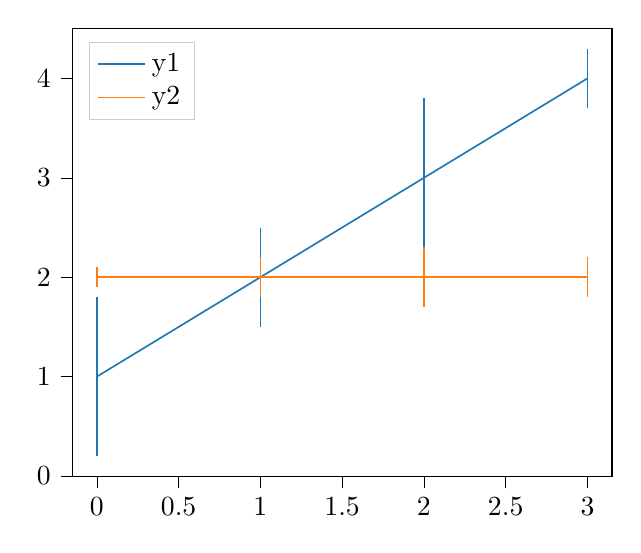
\begin{tikzpicture}

\definecolor{color0}{rgb}{0.12156863,0.46666667,0.70588235}
\definecolor{color1}{rgb}{1,0.49803922,0.054901961}

\begin{axis}[
legend cell align={left},
legend style={
  fill opacity=0.8,
  draw opacity=1,
  text opacity=1,
  at={(0.03,0.97)},
  anchor=north west,
  draw=white!80!black
},
tick align=outside,
tick pos=left,
x grid style={white!69.019608!black},
xmin=-0.15, xmax=3.15,
xtick style={color=black},
y grid style={white!69.019608!black},
ymin=-0.005, ymax=4.505,
ytick style={color=black}
]
\path [draw=color0, semithick]
(axis cs:0,0.2)
--(axis cs:0,1.8);

\path [draw=color0, semithick]
(axis cs:1,1.5)
--(axis cs:1,2.5);

\path [draw=color0, semithick]
(axis cs:2,2.2)
--(axis cs:2,3.8);

\path [draw=color0, semithick]
(axis cs:3,3.7)
--(axis cs:3,4.3);

\path [draw=color1, semithick]
(axis cs:0,1.9)
--(axis cs:0,2.1);

\path [draw=color1, semithick]
(axis cs:1,1.8)
--(axis cs:1,2.2);

\path [draw=color1, semithick]
(axis cs:2,1.7)
--(axis cs:2,2.3);

\path [draw=color1, semithick]
(axis cs:3,1.8)
--(axis cs:3,2.2);

\addplot [semithick, color0]
table {%
0 1
1 2
2 3
3 4
};
\addlegendentry{y1}
\addplot [semithick, color1]
table {%
0 2
1 2
2 2
3 2
};
\addlegendentry{y2}
\end{axis}

\end{tikzpicture}
